\documentclass{article}
\usepackage{tikz}
\usetikzlibrary{automata, positioning}
\begin{document}
	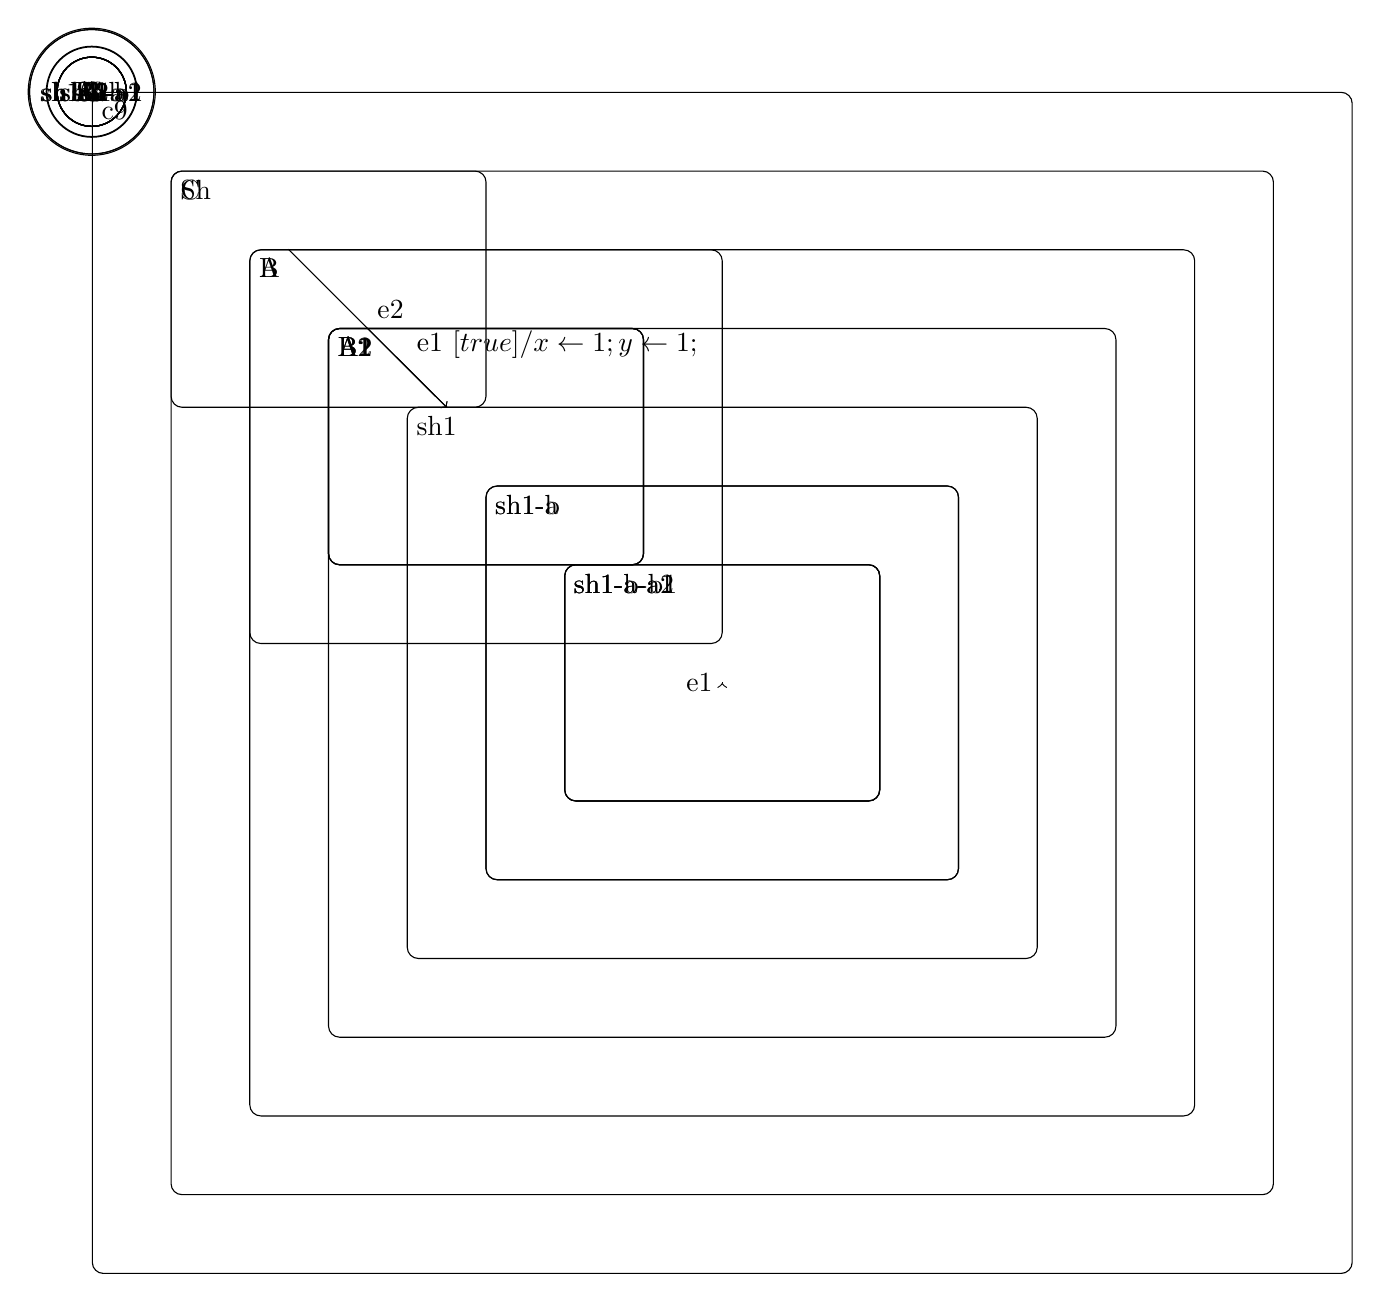
\begin{tikzpicture}[node distance=3cm, auto]
		\node[state] (c9) {c9};
		\node[draw, rectangle, rounded corners, minimum width=16cm, minimum height=15cm, anchor=north west, label={[anchor=north west] north west:c9}] (c9) at (0, 0) {};
		\node[state] (c9_Sh) {Sh};
		\node[draw, rectangle, rounded corners, minimum width=14cm, minimum height=13cm, anchor=north west, label={[anchor=north west] north west:Sh}] (c9_Sh) at (1, -1) {};
		\node[state] (c9_Sh_A) {A};
		\node[draw, rectangle, rounded corners, minimum width=12cm, minimum height=11cm, anchor=north west, label={[anchor=north west] north west:A}] (c9_Sh_A) at (2, -2) {};
		\node[state] (c9_Sh_A_A1) {A1};
		\node[draw, rectangle, rounded corners, minimum width=10cm, minimum height=9cm, anchor=north west, label={[anchor=north west] north west:A1}] (c9_Sh_A_A1) at (3, -3) {};
		\node[state] (c9_Sh_A_A1_sh1) {sh1};
		\node[draw, rectangle, rounded corners, minimum width=8cm, minimum height=7cm, anchor=north west, label={[anchor=north west] north west:sh1}] (c9_Sh_A_A1_sh1) at (4, -4) {};
		\node[state] (c9_Sh_A_A1_sh1_sh1_a) {sh1-a};
		\node[draw, rectangle, rounded corners, minimum width=6cm, minimum height=5cm, anchor=north west, label={[anchor=north west] north west:sh1-a}] (c9_Sh_A_A1_sh1_sh1_a) at (5, -5) {};
		\node[state] (c9_Sh_A_A1_sh1_sh1_a_sh1_a_a1) {sh1-a-a1};
		\node[draw, rectangle, rounded corners, minimum width=4cm, minimum height=3cm, anchor=north west, label={[anchor=north west] north west:sh1-a-a1}] (c9_Sh_A_A1_sh1_sh1_a_sh1_a_a1) at (6, -6) {};
		\node[state] (c9_Sh_A_A1_sh1_sh1_a_sh1_a_a2) {sh1-a-a2};
		\node[draw, rectangle, rounded corners, minimum width=4cm, minimum height=3cm, anchor=north west, label={[anchor=north west] north west:sh1-a-a2}] (c9_Sh_A_A1_sh1_sh1_a_sh1_a_a2) at (6, -6) {};
		\node[state] (c9_Sh_A_A1_sh1_sh1_b) {sh1-b};
		\node[draw, rectangle, rounded corners, minimum width=6cm, minimum height=5cm, anchor=north west, label={[anchor=north west] north west:sh1-b}] (c9_Sh_A_A1_sh1_sh1_b) at (5, -5) {};
		\node[state] (c9_Sh_A_A1_sh1_sh1_b_sh1_b_b1) {sh1-b-b1};
		\node[draw, rectangle, rounded corners, minimum width=4cm, minimum height=3cm, anchor=north west, label={[anchor=north west] north west:sh1-b-b1}] (c9_Sh_A_A1_sh1_sh1_b_sh1_b_b1) at (6, -6) {};
		\node[state] (c9_Sh_A_A2) {A2};
		\node[draw, rectangle, rounded corners, minimum width=4cm, minimum height=3cm, anchor=north west, label={[anchor=north west] north west:A2}] (c9_Sh_A_A2) at (3, -3) {};
		\node[state] (c9_Sh_B) {B};
		\node[draw, rectangle, rounded corners, minimum width=6cm, minimum height=5cm, anchor=north west, label={[anchor=north west] north west:B}] (c9_Sh_B) at (2, -2) {};
		\node[state] (c9_Sh_B_B1) {B1};
		\node[draw, rectangle, rounded corners, minimum width=4cm, minimum height=3cm, anchor=north west, label={[anchor=north west] north west:B1}] (c9_Sh_B_B1) at (3, -3) {};
		\node[state] (c9_Sh_B_B2) {B2};
		\node[draw, rectangle, rounded corners, minimum width=4cm, minimum height=3cm, anchor=north west, label={[anchor=north west] north west:B2}] (c9_Sh_B_B2) at (3, -3) {};
		\node[state] (c9_C) {C};
		\node[draw, rectangle, rounded corners, minimum width=4cm, minimum height=3cm, anchor=north west, label={[anchor=north west] north west:C}] (c9_C) at (1, -1) {};
		\draw[->] (c9_Sh_A_A2) edge node  {e1 {$[true]  / x \leftarrow 1; y \leftarrow 1;$}} (c9_C);
		\draw[->] (c9_Sh_B) edge node  {e2} (c9_C);
		\draw[->] (c9_Sh_A_A1_sh1_sh1_a_sh1_a_a1) edge node  {e1} (c9_Sh_A_A1_sh1_sh1_a_sh1_a_a2);
	\end{tikzpicture}
\end{document}
